%%
% Author Thomas C. Hales
% laTeX Format

%!TEX TS-program = latex    
%% This line is for TexShop. 

\documentclass[spanningrule]{cambridge7A}
%% Cambridge University Press Macros from
%% https://authornet.cambridge.org/information/productionguide/laTex_files/

% required by CUP
\usepackage[numbers]{natbib}
\usepackage{rotating}
\usepackage{floatpag}
 \rotfloatpagestyle{empty}
\usepackage{amsthm}
\usepackage{graphicx}
\usepackage{multind}\ProvidesPackage{multind}
\usepackage{times}

% my additions
\usepackage{verbatim}
\usepackage{latexsym}
\usepackage{amsfonts}
\usepackage{amsmath}
\usepackage{crop}
\usepackage{txfonts}
\usepackage[hyphens]{url}
\usepackage{setspace}
%\setstretch{2}  % for double spacing

% fonts
\usepackage[mathscr]{euscript} % powerset.
\usepackage{pifont} %ding
\usepackage[displaymath]{lineno}

%% hyperref interferes with the \part macro of cambridge
\usepackage[letterpaper,colorlinks=true,%
  citecolor=red,%
  %breaklinks=true,%
  %pdftex,
  ps2pdf,%
  hyperindex=true]{hyperref}

% Also interferes with \part macro of CUP.
% http://tug.ctan.org/tex-archive/macros/latex/contrib/pdfcomment/doc/pdfcomment.pdf
\usepackage{pdfcomment}

%%%%%%%%%%%%%%%%%%%%%%%%%%%%%%%%%%%%%%%%%

% This file contains local settings and system dependencies



% Auxiliary directories
\def\ps{../../../../Pictures/kep07ps}  % flypaper graphics
\def\pdf{/Users/thomashales/Pictures/collect_geom} % tarski graphics

\def\showgraphics{f}  
% t: display graphics (there are none to show yet)
% f (default): print a "no graphics logo" where graphics would normally go.


\def\displayallproof{t} 
% t (default): display all proofs.
% f: print documents without the proofs-- theorem statements only

\def\displayrating{f}
% t (default): display all ratings (verbose is also true)
% f : don't show them.

\def\verbose{f}
% f (default): do not display debugging information,
% t : display debug information and information about the formalization.

\def\tarskipagesep{f}
% f (default): no page breaks between lemmas in tarski collection.
% t :add page breaks

\def\tarskistrip{f}
% f (default): preserves control sequences in tarski collection
% t: control sequences in tarski collection are stripped and printed to an auxiliary file.

\def\tarskidump{f}
% t : dump tarski guid data to external write file.
% f (default) : don't use external write file.
 
%-%
% --Repository--
%-%
% generate revision number by
% svn propset svn:keywords "LastChangedRevision" kepmacros.tex
\def\svninfo{%
  TeXed on \today; \hfill\break
  Repository Root: https://flyspeck.googlecode.com/svn \hfill\break
  SVN $LastChangedRevision$
  }

%-%
% --Fonts--
%-%
\font\twrm=cmr8

%-%
% --Graphics--
%-%
%set \showgraphics option in flag_fly.tex
% flypaper graphics
\def\myincludegraphics#1{%
      \if\showgraphics t{\includegraphics{#1}}%
      \else{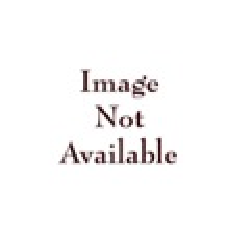
\includegraphics{noimage.eps}}\fi}
\def\szincludegraphics[#1]#2{%
      \if\showgraphics t{\includegraphics{#2}}%
      \else{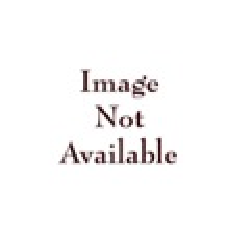
\includegraphics{noimage.eps}}\fi}

% kepler graphics
\def\pdffigtemplatex#1#2#3{%
\begin{figure}[htb]%
  \centering
  \myincludegraphics{\pdfp/#1}
  \caption{#3}
  \label{fig:#2}%
\end{figure}%
}
\def\pdfg#1#2#3{\if\showgraphics t{\pdffigtemplatex{#1}{#2}{#3}}\else{}\fi}


% tarski graphics
\def\pdffigtemplate#1#2#3{%
\begin{figure}[htb]%
  \centering
  \myincludegraphics{\pdf/#1}
  \caption{#3}
  \label{tarski:fig:#2}%
\end{figure}%
}
\def\pdffig#1#2#3{\if\showgraphics t{\pdffigtemplate{#1}{#2}{#3}}\else{}\fi}

%-%
% --Footnotes--
%-%
% http://help-csli.stanford.edu/tex/latex-footnotes.shtml
\long\def\symbolfootnote[#1]#2{\begingroup%
\def\thefootnote{\ensuremath{\fnsymbol{footnote}}}\footnote[#1]{#2}\endgroup}

%-%
% --Special Formatting--
%-%
% http://en.wikibooks.org/wiki/LaTeX/Formatting#List_Structures
\renewcommand{\labelitemii}{$\star$}


%-%
% --Indexing, References, Citations--
%-%
\def\indy#1#2{\index{index/#1}{#2}}

%-%
% --Proof Display--
%-%
% set with \displayallproof in flag_fly. If f, then proofs are swallowed.
%% "proved" environment. toggle with \displayallproof
%
\def\hide#1{}
\def\swallowed{\relax}
\def\swallow#1\swallowed{}
\newenvironment{iproved}{}{}
\newenvironment{proved}{\resetproved\begin{iproved}}{\end{iproved}}
\def\hideproof{\renewenvironment{iproved}{%
   \centerline{\it -- Proof Proofed --}
  \renewenvironment{itemize}{}{}
  \renewenvironment{enumerate}{}{}
  \def\item{\relax}
  \catcode13=12
  \swallow
}{}}
\def\showproof{\renewenvironment{iproved}{\begin{proof}}{\end{proof}}}
\def\resetproved{\if\displayallproof t\showproof\else\hideproof\fi}



%-%
% --Debugging Information--
%-%
\def\uf#1{{\par\narrower\it #1}} % unfinished manuscript
%% verbose:
\def\rating#1{\if\displayrating t{{\textsc {[rating={\ensuremath {#1}}].\ }}}\else{}\fi}
\def\oldrating#1{\if\displayrating t{{\textsc {[former rating={\ensuremath {#1}}].\ }}}\else{}\fi}
\def\formal#1{\if\verbose t{{\tt [formal: #1].\ }}\else{}\fi}
\def\formalauthor#1{\if\verbose t{{\tt [formal proof by: #1].\ }}\else{}\fi}
\def\footformal#1{\if\verbose t{\footnote{\formal{#1}}}\else{}\fi}
\def\usage#1{\if\verbose t{\symbolfootnote[1]{#1}}\else{}\fi}
\def\move#1#2{\begin{#1} See \ref{#2}.\end{#1}}
\def\FIXX#1{\if\verbose t{\footnote{\tt [#1]}}\else{}\fi}
\def\page#1#2{#2 {\it [dcgp.#1]}}
% first entry Lemma or Sec of DCG, second entry page.
\def\dcg#1#2{{\if\verbose t{{\tt{[DCG-#1]}}\indy{References}{ZC{#2 #1}@{DCG-#1}|page{#2}}}\else{}\fi}}
\def\tlabel#1{\label{#1}\if\verbose t{{\tt [#1].\ }%
   \indy{References}{#1|itt}}\else{}\fi}
\def\ifverbose#1{\if\verbose t{{#1}}\else{}\fi}




%% Indexing
\def\refXX{0} % for unknown links.
\def\showref#1{\ref{#1}{\tt[#1]}\indy{References}{#1}}
\def\oldlabel#1{\label{x-#1}}

\def\tref#1{\ref{#1}\indy{References}{#1}}
\def\itt#1{{\bf #1}}
\def\guid#1{{\tt[#1].\ }\indy{References}{ZA{#1}@{#1}|itt}}
% textsc
\def\calc#1{{\textsc{calc-#1}}\indy{Interval}{{#1}@{#1}}}
\def\newcalc#1{{\textsc{newcalc-#1}}\indy{Interval}{{#1}@{#1 (new XX)}}}
\def\assembly#1{{\textsc{assembly-#1}}\indy{References}{ZD{#1}@{#1}}}
%\def\conseq#1{{\textsc{conseq-#1}}}

%% 


%% Tarski indexing. Write summary data to external file "\mywrite",
% which is generated in tarski.tex
% Need to extend cs character set.  Use this only within a block.
\def\setcat{
\catcode`\-=11
\catcode`\.=11
\catcode`\:=11
\catcode`\0=11
\catcode`\1=11
\catcode`\2=11
\catcode`\3=11
\catcode`\4=11
\catcode`\5=11
\catcode`\6=11
\catcode`\7=11
\catcode`\8=11
\catcode`\9=11
}
\def\tarfe#1#2{{\foote{{\tt[L.E.G:#1]}~\csname #1-sum\endcsname%
  \expandafter\ifx \csname #1-guid\endcsname \relax [XX-BAD-IDENTIFIER]\else{}\fi
  }
  {\csname #1-guid\endcsname{#2}}}}
\def\tarf#1{\tarfe{#1}{}}
\def\tarfE#1{\tarfe{EE}{-\csname #1\endcsname}}
% control sequences will contain [-.0-9:] \catcode`\-=11, etc.
\newtoks\mysummary
\newtoks\myguid
\newtoks\myname
\def\separator{\if\tarskipagesep t{\clearpage}\else%
  \smallskip\hrule height 0.5pt depth 0pt width 60pt\bigskip\fi}
\def\identity#1{#1}
\def\foote#1#2{\footnote{#1~{\it (#2)}}}
\def\marker#1#2{\par\hangafter1\hangindent=1em\noindent{\bf #1:}\quad #2}
\def\name#1{\marker{Name}{#1}\myname={#1}
  \write\myhtml{  "#1", //name}
}
\def\summary#1{\marker{Summary}#1\mysummary={#1}
  % cleanse control sequences for html
  \if\tarskistrip t{
  \def\sqr{sqrt}
  \def\sqrt{sqrt}
  \def\op{\identity}
  \def\epsilon{epsilon}
  \def\Delta{Delta}
  \def\ups{upsilon}
  \def\beta{beta}
  \def\rho{rho}
  \def\CalE{E}
  \def\chi{chi}
  \def\eta{eta}
  \write\myhtml{  "#1", // summary}
  }
  \else\relax\fi
}
\def\guid#1{\if\tarskidump f{{\tt [#1]}}\else{\marker{ID}#1
   \indy{guid}{#1}
   \immediate\write\mywrite{\global\expandafter\def\csname \the\myname-sum \endcsname{\the\mysummary}}
   \immediate\write\mywrite{\global\expandafter\def\csname \the\myname-guid \endcsname{#1}}
   \immediate\write\myhtml{  "#1" // guid}}%
   \fi
}
\def\tag#1{\marker{Tags}#1
   \immediate\write\myhtml{  "#1", // tag}
}
%\def\rating#1{\marker{Rating}#1
%   \write\myhtml{  <rating>#1</rating>}
%}
\newenvironment{tarski}{%
\write\myhtml{new Tarski(}
%\def\name   {\marker{Name}}
%\def\summary{\marker{Summary}}
%\def\tag    {\marker{Tags}}
\def\rating {\marker{Rating}}
\def\hol{\marker{HOL-Light}}
%\def\guid   {\marker{ID}}
\def\tlabel{\label}
}{\separator\immediate\write\myhtml{),}
}
\newenvironment{tarskidata}{\write\myhtml{var tarskis=[}}
{
\immediate\write\myhtml{];}
}
%% tarski indexing
%\def\tarf#1{\footnote{{\tt geom-#1~\ref{#1}}\indy{ZA{#1}@{#1}}}}




%-%
% --Symbols--
%-%
% norm
\def\|{{\hskip0.1em|\hskip-0.15em|\hskip0.1em}}
\def\mid{\ :\ }
\def\norm#1#2{\|#1 - #2\|}
\def\normo#1{{\|#1\|}}
\def\sland{\ \land\ }
% Sam's
\def\myscorept{\text{ \sl pt}}
\def\qrtet{{quasi-regular tetrahedron}}
\def\qrtets{{quasi-regular tetrahedrons}}
\def\tomcite{{}}
\DeclareMathOperator{\myscore}{\sigma}
 \DeclareMathOperator{\gma}{gma}
 \DeclareMathOperator{\score}{\sigma}
 \DeclareMathOperator{\sol}{sol}
 \DeclareMathOperator{\dih}{dih}
\newtheorem{calcf}{Calculation}[subsection]

% mathcal
\def\CalB{{\mathcal B}}
\def\CalC{{\mathcal C}}
\def\CalD{{\mathcal D}}
\def\CalE{{\mathcal E}}
\def\FF{{\mathcal F}}
\def\CalF{{\mathcal F}}
\def\CalQ{{\mathcal Q}}
%\def\CalW{{\mathcal W}}
\def\CalR{{\mathcal R}}
\def\CalS{{\mathcal S}}
\def\CalV{{\mathcal V}}
\def\T{{\mathcal T}}
\def\Q{{\mathcal Q}}


% brackets
\def\leftopen{]}
\def\leftclosed{[}
\def\rightopen{[}
\def\rightclosed{]}

%% obsolete
\def\leftb{[}
\def\rightb{]}

% squiqqly relations
\def\seq{\approx}
\def\sle{\preceq}
\def\sge{\succeq}
\def\slt{\prec}
\def\sgt{\succ}

% mathbb
\def\R{{\mathbb R}}
\def\N{{\mathbb N}}
\newcommand{\ring}[1]{\mathbb{#1}}
\def\A{{\mathbf A}}
\def\Rp{\ring{R}^{3\,\prime}}

% operatorname
\def\op#1{{\operatorname{#1}}}
\def\optt#1{{\operatorname{{\texttt{#1}}}}}

\def\opat{\op{@}}
\def\atn{\op{arctan\ensuremath{_2}}}
\def\azim{\op{azim}}
\def\sol{\operatorname{sol}}
\def\vol{\op{vol}}
\def\quo{\operatorname{quo}}
\def\anc{\operatorname{anc}}
\def\cro{\operatorname{crown}}
%\def\vor{\operatorname{vor}}
%\def\svor{\operatorname{svor}}
\def\sign{\operatorname{sign}}
\def\octavor{\operatorname{octavor}}
\def\dih{\operatorname{dih}}
\def\Adih{\operatorname{Adih}}
\def\arc{\operatorname{arc}}
\def\cosarc{\operatorname{cosarc}}
\def\rad{\operatorname{rad}}
\def\gap{\operatorname{gap}}
\def\sc{{\operatorname{sc}}}
\def\geom{{\operatorname{g}}}
\def\anal{{\operatorname{an}}}
\def\PM{\operatorname{PM}}
\def\bool{\operatorname{bool}}
\def\true{\op{true}}
\def\false{\op{false}}
\def\flat{\operatorname{flat}}
\def\tangle#1{\langle #1\rangle}
\def\ceil#1{\lceil #1\rceil}
\def\floor#1{\lfloor #1\rfloor}
\def\ups{\upsilonup} % Needs txfonts; else use \upsilon
\def\orgn{\varthetaup} % center of packing
%\def\comp#1{\llbracket #1 \rrbracket}
\def\comp#1{[#1]}
\def\Wdart{W_{\text{dart}}}
\def\Wedge{W_{\text{edge}}}
\def\cell{\operatorname{cell}}

\def\SA{A}
\def\SB{B}
\def\SC{C}
\def\SD{D}
\def\SE{E}
\def\del{\partial}
\def\doct{\delta_{oct}}
\def\dtet{\delta_{tet}}
\def\pt{\hbox{\it pt}}
\def\hm{{h_0}} % 1.26
%\def\Vol{\hbox{vol}}
\def\scoregoal{8\,\pt}
\def\maxpi{\pi_{\max}}
\def\tausc{{\tau\!\operatorname{sc}}}
\def\piF{{\pi_F}}
\def\xiG{\xi_\Gamma}
\def\piG{\pi_\Gamma}
\def\xiV{\xi_V}
\def\xik{\xi_\kappa}
\def\xikG{\xi_{\kappa,\Gamma}}
\def\piV{\pi_V}
\def\tauLP{{\tau_{\hbox{\twrm LP}}}}
\def\DLP{\operatorname{D}_{\hbox{\twrm LP}}}
\def\ZLP{\operatorname{Z}_{\hbox{\twrm LP}}}
\def\tlp{\tau_{\hbox{\twrm LP}}}  % 2 args (p,q) tri, quad
\def\sLP{\sigma_{\hbox{\twrm LP}}}  % 2 args (p,q) tri, quad
\def\squander{(4\pi\zeta-8)\,\pt}
\def\trgt{\operatorname{\it{target}}}
\def\tildeF{{\hbox{$\tilde F$}}}
\def\zloop{{z}_{loop}}
\def\dloop{{\delta}_{loop}}
\def\sqr{\sqrt}
\def\tildeV{V^{\CalS}}
%\def\BigD{\Delta}
%\def\bigd{\Delta^0}
\def\FCinner{\op{FC}_{\text{inner}}}
\def\FC{\op{FC}}
\def\FCR{\op{FCR}}
\def\rogFC{\op{rog}^0_{\text{FC}}}
\def\chino{\chi_0}

\def\x#1{\op{\bf c}{#1}}  % marks context \x(p,r).
\def\xs#1{\op{\bf sc}{#1}}  % marks special context \x(p,r,s).
\def\xtazimlt{\x{(3,1: \op{azim}(\op{gap}) <\pi)}}
\def\xtazimge{\x{(3,1: \op{azim}(\op{gap}) \ge \pi)}}
\def\xfgap{\x{(4,1:\op{gap})}}
\def\y#1{\op{\bf ep}{#1}}  % marks edge parameters \y(n,k).
\def\pqr#1{#1} % marks type (p,q,r).
%\def\pqr#1{\op{\bf typ}{#1}} % marks type (p,q,r).

%% HYPERMAP macros:
% avoid e for both hypermap edge and edge {v,w}
\def\e{\varepsilonup}
\def\ocirc{}



%% FORMULATION macros:
\def\lam{\lambda}
\def\Lam{\Lambda}
\def\bl{{\underline{\lam}}}
\def\bm{{\underline{\mu}}}
\def\angle#1#2#3{{\op{angle}(#1,{#2,#3})}}


\def\card{\op{card}}

% accent used in India citation in Overview.
\def\=#1{\accent"16 #1}
\def\i{I}
%\def\={\relax}



%% Enclosed CALE control sequences:
\expandafter\def\csname 2t0-doesnt-pass-through\endcsname{01}
\expandafter\def\csname E1453\endcsname{02}   
\expandafter\def\csname dcg-p89\endcsname{03}   
\expandafter\def\csname enclosed-v\endcsname{04}   
\expandafter\def\csname 277\endcsname{05}   
\expandafter\def\csname 245\endcsname{06}   
\expandafter\def\csname 245bis\endcsname{07}   
\expandafter\def\csname node\endcsname{08}   
\expandafter\def\csname E:part4:1\endcsname{09}   
\expandafter\def\csname E:part4:2\endcsname{10}   
\expandafter\def\csname E:part4:3\endcsname{11}   
\expandafter\def\csname E:part4:4\endcsname{12}   
\expandafter\def\csname E:part4:5\endcsname{13}   
\expandafter\def\csname E:part4:6\endcsname{14}   
\expandafter\def\csname E:part4:7\endcsname{15}   
\expandafter\def\csname E:part4:8\endcsname{16}   
\expandafter\def\csname E:part4:9\endcsname{17}   
\expandafter\def\csname E:part4:10\endcsname{18}   
\expandafter\def\csname dcg-p142\endcsname{19}   
\expandafter\def\csname convex-quad\endcsname{20}   
\expandafter\def\csname last:E\endcsname{21}
\expandafter\def\csname rem2.7\endcsname{22}     
\expandafter\def\csname pass-anchor\endcsname{23}

%% 
 
 
 
 
 
 
 


% line numbers
\def\lll{\resetlinenumber[1]}
\def\linenumberfont{\normalfont\small\sffamily}

\def\tocpart#1{
  \addcontentsline{toc}{part}{\Large{#1}}}
% (or even \LARGE)
  
\crop
%\makeindex
\makeindex{index/Notation}
\makeindex{index/Index}

\def\linput#1{\lll\input{#1}}


\raggedbottom  % for now.
%\raggedright  % don't worry for now.

%%% end notes -kill this.
%%\maketextnotes

%%%%%%%%%%%%%%%%%%%%%%%%%%%%%%%%%%%%%%%%

% new theorems

\theoremstyle{plain}
\newtheorem{theorem}[equation]{Theorem}
\newtheorem{lemma}[equation]{Lemma}

\newtheorem{background}[equation]{Background}
\newtheorem{corollary}[equation]{Corollary}
\newtheorem{example}[equation]{Example}
\newtheorem{assumption}[equation]{Assumption}
\newtheorem{interpretation}[equation]{Interpretation}
\newtheorem{conjecture}[equation]{Conjecture}

\theoremstyle{definition}
\newtheorem{definition}[equation]{Definition}

\theoremstyle{remark}
\newtheorem{remark}[equation]{Remark}
\newtheorem{notation}[equation]{Notation}
%\newtheorem{note}[equation]{Author's Note}
\newtheorem*{note}{Author's Note.}
\newtheorem{calculation}[equation]{Calculation}
\newtheorem{assertion}[equation]{Assertion}
\newtheorem{exer}[equation]{Exercise}

%%%%%%%%%%%%%%%%%%%%%%%%%%%%%%%%%%%%%%%%%

\begin{document}
\title[for {\it Dense Sphere Packings}]{Software Guide}
\author{Thomas C. Hales}
    
%%%%%%%%%%%%%%%%%%%%%%%%%%%%%%%%%%%%%%%%%
%%% FRONT
    \frontmatter
    \maketitle
    \tableofcontents

%%%%%%%%%%%%%%%%%%%%%%%%%%%%%%%%%%%%%%%%%

   \newpage
 
%%%%%%%%%%%%%%%%%%%%%%%%%%%%%%%%%%%%%%%%%
  \mainmatter
  \begin{runninglinenumbers*}

\chapter{Nonlinear Programming Software}

\newterm{Nitpick} comes from the acronym NPK for Nonlinear Programming for the Kepler conjecture.

The following resources are available for the proof of nonlinear inequalities.  The years of active development are indicated.

\begin{itemize}
\item Roland Zumkeller's 
Sergei software%
\footnote{\url{http://code.google.com/p/sergei/}} %
 2008-2010.
\item Sean McLaughlin's KeplerCode software%
\footnote{\url{http://code.google.com/p/kepler-code/}}%
\item Sam Ferguson's software \url{}, 1994--1998.
\item Thomas Hales's software \url{}, 1994--1998.
\end{itemize}

Some chapters in this guide give details about the specific nonlinear inequalities that are
used in {\it Dense Sphere Packings}.

The following resources are available for the nonrigorous verification of inequalities.

\begin{itemize}
\item 
\end{itemize}

\chapter{Linear Programming Software}

The following resources are available for linear programming for {\it Dense Sphere Packings}.

\begin{itemize}
\item Steven Obua's software \url{}.
\item \newterm{Lipstick} software \url{}.
\end{itemize}

\section{Flyspeck II}

Steven Obua's thesis shows how to treat $92.5\%$ of the tame graphs
that appear in the original proof of the Kepler conjecture~\cite{obua:phd}.  There are
several additional sources of documentation including a 50 minute video
presentation by Obua at Lausanne in 2008~\cite{obua:2008:video} and a
published account by Obua and Nipkow~\cite{obua-nipkow:2009}.

\section{Lipstick}

The Lipstick program takes its name from the acronym LPSK, for
{\it Linear Programming Software for the Kepler conjecture}.  It is available
at the google code svn repository for the Flyspeck project.


\subsection{google code download}\label{sec:google-code}

To download code from google code, \newterm{subversion}\footnote{\url{http://subversion.apache.org/}} (svn) must be
installed on your computer.  Please install if necessary before continuing.

There are no precompiled binaries for the project.  The source code
must be downloaded and then compiled.  This subsection gives
instructions about how to download source code.

To download code from a google code project go to the main page of the
project, click on the source tab, then the checkout tab, then follow
the instructions.

For example to download the entire Flyspeck project, go to
the Flyspeck project%
\footnote{\url{http://code.google.com/p/flyspeck/}} % 
click the source and
checkout tabs to arrive at the checkout%
\footnote{\url{http://code.google.com/p/flyspeck/source/checkout}} % 
 page.
That page
lists the following command to anonymously check out the source code:
\begin{verbatim}
svn checkout http://flyspeck.googlecode.com/svn/trunk/ 
  flyspeck-read-only
\end{verbatim}

It is possible to check out part of the project.  For example to get
the linear programming part of the project
\begin{verbatim}
svn checkout http://flyspeck.googlecode.com/svn/trunk/glpk/ 
  glpk-read-only
\end{verbatim}

\subsection{installation}

The lipstick code is available from the Flyspeck google code repository in
the glpk%
\footnote{\url{http://flyspeck.googlecode.com/svn/trunk/glpk}} %
 subdirectory.  Section~\ref{sec:google-code}
gives instructions for downloading code from the google code repository.

The following other resources are needed to run the code.

\begin{itemize}
\item The Objective Caml language%
\footnote{\url{http://caml.inria.fr/}} %
\item The GNU Linear Programming Kit (GLPK)%
\footnote{\url{http://www.gnu.org/software/glpk/}} %
\item The archive of tame graphs% 
\footnote{\url{http://weyl.math.pitt.edu/hanoi2009/Kepler/Kepler}}
\end{itemize}

The code uses the GNU MathProg modeling language to describe the linear programs that arise in the proof of the Kepler conjecture.

The following sources of documentation are useful.

\begin{itemize}
\item Modeling Language GNU MathProg manual.  This manual is part of the GLPK distribution.  It is also directly downloadable in pdf%
\footnote{\url{http://www.cs.unb.ca/~bremner/docs/glpk/gmpl.pdf} --2008 version} %
 and html%
\footnote{\url{http://www.im.pwr.wroc.pl/~przemko/opty/gmpl.html}} %
\end{itemize}


\chapter{Graph Generator Software}


\begin{itemize}
\item The Nipkow-Bauer Flyspeck I project.
\item Gangplank software
\end{itemize}

\section{Flyspeck I}

The Flyspeck I project makes a formal verification of the enumeration
of tame graphs that appear in the original proof of the Kepler
conjecture~\cite{BauerN-AFP06}.  The project started with Bauer's
thesis under the direction of Nipkow~\cite{Bauer:2006:Thesis}.  The
formal verification was done in the Isabelle proof assistant.  The
code is available~\cite{BauerN-Flyspeck-I-Isabelle}.

In 2009, it became necessary to change some of the parameters that enter into the definition of tame graph.  This requires minor changes to the Flyspeck I project.



\section{Gangplank}

The name \newterm{Gangplank} comes from the acronym GGPK for the {\it
  Graph Generation Program for the Kepler conjecture.}  Gangplank is a
program written in Java for the generation of restricted hypermaps with special properties.
The first version of the software was written by Hales in 1994.  It
has been under gradual development by him since then.

A set of input parameters defines a class $C$ of restricted hypermaps.  Gangplank
then generates a list $D$ of hypermaps with the property that every hypermap in $C$
appears in $D$, up to unoriented\footnote{Hypermaps $H$ and $H'$ have
an unoriented isomorphism between them if $H$ is isomorphic to $H'$ or
$H$ is isomorphic to the opposite of $H'$.} isomorphism.

In practice, it may be difficult to check whether some of the properties of  a hypermap
are satisfied.  Gangplank is conservative in its approach.  If in doubt, it prints it out.
This means that the list $D$ may contain extraneous hypermaps.

\subsection{installation and execution}

The software is available in the graph\_generator%
\footnote {\url{http://flyspeck.googlecode.com/svn/trunk/graph_generator}} %
 directory at the flyspeck google code repository.  Section~\ref{sec:google-code} gives instructions on downloading the code.

The Java%
\footnote{\url{http://www.java.com/}} %
 programming language must be installed on the computer for the software to run.

To compile Gangplank:

\begin{itemize} 
\item Open a shell, 
\item Change into the graph\_generator/src subdirectory
\item Type the following command at the shell prompt:
\begin{verbatim}
javac -d ../classes graph/Generator.java 
\end{verbatim}
\end{itemize}

To run Gangplank:

\begin{itemize}
\item Choose a properties file from the graph\_generator/properties subdirectory and copy it to /tmp/graph.properties.  (The behavior of the program is directed by this file.)
\item Change into the subdirectory graph\_generator/classes
\item Type the following command at the shell prompt:
\begin{verbatim}
java -Xms300m -Xmx1g graph/Generator  
\end{verbatim}
\end{itemize}

The output goes to the standard output (screen).

\subsection{terminology}

This section follows the terminology from {\it Dense Sphere Packings}.  In particular,
it uses the language of hypermaps.  An exceptional face of a hypermap is one with
at least five darts.  The type of a node is a triple $(p,q,r)$,
where $p$ is the number of triangles that meet the node, $q$ is the number of quadrilaterals that meet it, and $r$ is the number of exceptional faces that meet it.
A node is a set of darts. Its cardinality corresponds to what is called the degree of the
node in graph theory.

\subsection{input parameters}

The input parameters are given in a file /tmp/graph.properties.
(To use a different input file, edit the string propertiesFile
in src/graph/Constants.java.)  Various examples of properties files
are found in the directory graph\_generator/properties.

The format of the properties file is a Java configuration%
\footnote{\url{http://en.wikipedia.org/wiki/.properties}} % 
file.  A line beginning with \verb!#! or ! is interpreted as a comment.
Each property is given by a line of the form key=value.
Most parameters have a default value if none is specified.
This subsection describes the keys, admissible values, and defaults.
Each choice of parameters describe a class of restricted hypermaps, which we will call $C$.
(A better notation would show the dependence of $C$ on the parameters:
$C(\text{excludeDegree2,excludePentQRTet},\ldots)$, but this would be unwieldy.)
The program Gangplank generates a set of hypermaps that contains every element of
$C$ up to unoriented isomorphism.


\subsubsection{excludeDegree2=false}

If set to true,  $C$ does not contain any hypermaps with a vertex of degree $2$.

\subsubsection{excludePentQRTet=false}

If set to true,  $C$ does not contain a hypermap with a node of type $(1,0,1)$
in which the exceptional face is a pentagon. (See Figure~\ref{fig:excludePentQRTet}.)

\tikzfig{excludePentQRTet}
{If true, the node $3$ of type $(1,0,1)$ is excluded.}
{
[scale=0.004]
% java render/Gentikz "33 4  4 0 4 2 1 4 0 1 2 3    3 2 4 3     3 0 3 4 "
%tikz format auto generated by Gentikz
%in LaTeX file, enclose code in tikzpicture environment
% invariant: 147615209765
%Set the coordinates of the points:
\tikzstyle{every node}=[draw,shape=circle];
\path ( 400,0) node (P0) {$0$};
\path ( 0,-400) node (P1) {$1$};
\path ( -400,0) node (P2) {$2$};
\path ( 0,0) node (P3) {$3$};
\path ( 0,400) node (P4) {$4$};
%Draw edges:
\draw
  (P0) -- (P1)
  (P0) -- (P4)
%  (P0) -- (P3) % hand edited.
  (P1) -- (P2)
  (P2) -- (P4)
  (P2) -- (P3)
  (P3) -- (P4)
;
}

\subsubsection{exclude2inQuad=true}

If set to true, then $C$ does not contain a  hypermap that contains a
simple contour loop through precisely four nodes such that both the interior and exterior
 contain at least two additional nodes. (See Figure~\ref{fig:exclude2inQuad}.)
Expressed in terms of planar graphs, there is no $4$-cycle such that both its interior
and exterior contain at least two nodes.

\tikzfig{exclude2inQuad}
{If true, $C$ does not contain this subarrangement.}
{
[scale=0.004]
% java render/Gentikz "33 2 4 0 1 2 3 4 0 3 2 1"
% nodes P4,P5,P6,P7 added by hand.
%tikz format auto generated by Gentikz
%in LaTeX file, enclose code in tikzpicture environment
% invariant: 230148743091
%Set the coordinates of the points:
\tikzstyle{every node}=[draw,shape=circle];
\path ( 400,0) node (P0) {$0$};
\path ( 0,400) node (P1) {$1$};
\path ( -400,0) node (P2) {$2$};
\path ( 0,-400) node (P3) {$3$};
\path (-100,0) node (P4) {$4$};
\path (100,0) node (P5) {$5$};
\path (-300,300) node (P6) {$6$};
\path (300,300) node (P7) {$7$};
%Draw edges:
\draw
  (P0) -- (P3)
  (P0) -- (P1)
  (P1) -- (P2)
  (P2) -- (P3)
;
}


\subsubsection{exclude1inTri=true}

If set to true, then $C$ does not contain a  hypermap that contains a
contour loop through precisely three nodes such that both the interior and exterior
contain both contain at least one additional node.  (See Figure~\ref{fig:exclude1inTri}.)

\tikzfig{exclude1inTri}
{If true, $C$ does not contain this subarrangement.}
{
[scale=0.004]
%tikz format auto generated by Gentikz
%in LaTeX file, enclose code in tikzpicture environment
%Set the coordinates of the points:
\tikzstyle{every node}=[draw,shape=circle];
\path ( 400,0) node (P0) {$0$};
\path ( -200,346) node (P1) {$1$};
\path ( -200,-346) node (P2) {$2$};
\path (0,0) node (P3) {$3$};
\path (300,300) node (P4) {$4$};
%Draw edges:
\draw
  (P0) -- (P2)
  (P0) -- (P1)
  (P1) -- (P2)
;
}

\subsubsection{ignoreArchive=false}

There is a large archive of hypermaps /src/graph/archive.java.  Let $D$ be this
collection.   When true,
the list of hypermaps in the archive is ignored and all hypermaps are built from scratch.

When false, the class $C$ is effectively replace with $C\setminus D$.  The output
of Gangplank only reports hypermaps that are outside the archive.

This parameter differs from the others because it affects the output, rather than the
definition of the class $C$.

\subsubsection{vertexCountMin=1}

For every hypermap $H$ in $C$, the number of nodes of $H$ is at least this value.
The value must be at least $0$.  The class $C$ is empty unless the value is at least $3$.

\subsubsection{vertexCountMax=100}

For every hypermap $H$ in $C$, the number of nodes of $H$ is at most this value.
This value must be at least vertexCountMin.

\subsubsection{nodeCardMaxAtExceptionalVertex=5}

For every hypermap $H$ in $C$, the cardinality of every node with an exceptional face
is at most this value.

\subsubsection{nodeCardMax=6}

For every hypermap $H$ in $C$, the cardinality of every node is at most
this value.  The name of the parameter is not very intuitive.  In
graph theory terms, it is the upper bound on the degree of a vertex.

\subsubsection{faceCardMax=8}

For every hypermap $H$ in $C$, the cardinality of every face is at most
this value.  

\subsubsection{squanderTarget=1}

The next few parameters relate to admissible weight assignments.  A
weight assignment on a hypermap is a real-valued function on its set
of faces.  The admissibility conditions are given as a system of
inequalities on the weight assignment.  These conditions depend on parameters
$a,b,d,k,\op{tgt}$.

The parameter $\op{tgt}$ equals squanderTarget, and $k$ equals 
nodeCardMaxAtExceptionalVertex.  The other three parameters are functions:
$a:\ring{N}\to\ring{R}$, $b:\ring{N}^2\to \ring{R}$ and $d:\ring{N}\to\ring{R}$.
A weight assignment $\tau$ on a hypermap $H$
is $(a,b,d,k,\op{tgt})$-\newterm{admissible}, if the following
conditions hold.
\begin{enumerate}
\item \case{total weight} $\sum_F \tau(F) < \op{tgt}$.
\item \case{bound~a} 
Let $v$ be any node of type $(p,q,r)$ such that $p+q+r=k$ and $r>1$. Let
  $A$ be the set of triangles and quadrilaterals meeting that node.  Then
\[ \sum_{F\in A} \tau(F)
\ge  a(p) + p\, d(3) + q\, d(4).\] 
\item \case{bound~b}
\formaldef{}{adm\_2}
 If a node $v$ has type $(p,q,0)$, then%
\footnote{The conditions in the original proof of the Kepler conjecture were slightly
more complicated than this, being expressed on \newterm{separated} sets of nodes.  Early versions of Gangplank had to treat this more general condition.}
  \[ \sum_{F:\,v\cap F\ne\emptyset} \tau(F) \ge
    b(p,q).\] 
%        \label{admissible:b}
\item \case{bound~d}
\formaldef{}{adm\_1}
 If the face $F$ has cardinality $n$, then
$\tau(F) \ge d(n)$.
\end{enumerate}
Note that for each $p$ and constant $a(p)$ there are various vertex types that go with it:
\[
(p,0,k-p),\quad (p,1,k-p-1),\ldots,\quad (p,k-1-p,1).
\]


The admissibility parameters $a,b,d$ are defined in the configuration
file.  Every hypermap $H\in C$ must have an
$(a,b,d,k,\op{tgt})$-admissible weight assignment for the
given parameters.

\begin{example}  If $\op{tgt}=1$ and the functions $a,b,d$ are all identically zero,
then the zero function is an admissible weight assignment.  This choice of parameters
effectively 
turns the weight assignment conditions off.
\end{example}

\begin{example} If  $d(n)\ge\op{tgt}$ for some $n$, then a hypermap with
an admissible weight assignment cannot have a face of cardinality $n$.  This gives
a way to constrain the sizes of the faces.
\end{example}

\begin{example} If $b(p,q)\ge\op{tgt}$ for some $(p,q)$, then a hypermap with
an admissible weight assignment cannot have a node of type $(p,q,0)$.  This gives
a way to constrain the types of the vertices.
\end{example}

\subsubsection{tableWeightD\wild =squanderTarget}

These parameters set the function $d$ that is used to define admissibility.
The default is the squander target, which means that a face of that size cannot occur
in the class $C$.

\begin{example} Suppose the properties file contains the following lines:
\begin{verbatim}
squanderTarget=1600
tableWeightD3=0
tableWeightD4=200
tableWeightD5=400
tableWeightD6=900
\end{verbatim}
Faces of other sizes are assigned the default $\op{tgt}$, 
which means they cannot occur.  
For these parameters, 
we may deduce that
every hypermap $H$ in the class $C$ has the following properties:
\begin{itemize}
\item Every face has $3,4,5$ or $6$ sides.
\item There cannot be two hexagons: $2d(6) =1800 > 1600=\op{tgt}$.
\item A hypermap with one hexagon has at most one pentagon: $d(6)+2d(5) = 1700 > 1600 = \op{tgt}$.
\end{itemize}
\end{example}
Property declarations 
that are not in the range $n=3,\ldots,\text{faceCardMax}$ are ignored.
The constants are required to be monotonic:
\[
d(3) \le d(4) \le \cdots
\]

\subsubsection{tableWeightA\wild =squanderTarget}

These parameters set the function $a$ that is used to define admissibility.
The default is the squander target, which means that a face of that size cannot occur
in the class $C$.

\begin{example} Suppose the properties file contains the following lines:
\begin{verbatim}
squanderTarget=1500
nodeCardMaxAtExceptionalVertex=6
tableWeightD3=0
tableWeightD4=200
tableWeightD6=700
tableWeightA5=800
\end{verbatim}
Suppose there is a node of type $(5,0,1)$. The associated constants
are $p=5,q=0,r=1,k=p+q+r=6$.
Let  $A$ be the set of five triangles at that node.  The definition of admissible
weight assignment implies that
\[
\sum_{F\in A}\tau(F) \ge a(5) + 5\, d(3) + 0\, d(4) = a(5) = 800.
\]
We conclude that a hypermap in class $C$ cannot contain both a node of type $(5,0,1)$
and a hexagon: 
\[
800 + d(6) = 1500 = \op{tgt}.
\]
\end{example}

\begin{example}
At a node of type $(0,0,k)$, the condition is
\[
0  =\sum_{F\in\emptyset}\tau(F) \ge a(0),
\]
which is inconsistent unless $a(0)\le 0$.  This means that if $a(0)$ is set to any
positive value, the class $C$ does not contain any nodes of type $(0,0,k)$.
In particular, if the default value is used and $\op{tgt}$ is positive, then no nodes
of type $(0,0,k)$ occur.
\end{example}

Property declarations 
that are not in the range 
\[
p=0,\ldots,\text{nodeCardMaxAtExceptionalVertex}-1
\]
are ignored. 


\subsubsection{tableWeightB\wild\wild=squanderTarget}

These parameters set the function $b$ that defines admissibility.  The default is
the squander target, which means that a vertex of that type $(p,q,0)$ cannot occur in
$C$.

\begin{example} Suppose the properties file contains the following lines:
\begin{verbatim}
squanderTarget=1600
tableWeightB21= 800
tableWeightB22= 400
tableWeightB23=1200
\end{verbatim}
From the definition of admissibility, it follows that if a node of type $(p,q,0)$ occurs,
then $p=2$ and $q\in\{1,2,3\}$.  Moreover, there are various restrictions on 
combinations of nodes.  For example, there cannot be two nodes of type $(2,1,0)$ because
$2b(2,1)  = 1600=\op{tgt}$.
\end{example}
Properties declarations where $p$ or $q$ is greater than nodeCardMax are ignored.

\subsubsection{tableWeightC}

In the specification of admissibility, there are functions $a,b,d$,
but no function $c$.  This happens for historical reasons.  There was
originally a function $c$ that was similar in purpose to $d$, but it
has been retired.

\subsection{archive format}

The output consists of strings that encode the combinatorial structure of planar graphs.  (More precisely, the strings encode planar hypermaps.)

Here is a sample string:
\begin{verbatim}
65974205892 19 4 0 1 2 3 4 0 3 4 5 3 4 3 6 3 6 
3 2 3 6 2 7 3 7 2 8 3 8 2 1 3 8 1 9 4 9 1 0 5 
3 9 5 10 3 10 5 4 3 10 4 11 3 11 4 6 3 11 6 7 
3 11 7 12 3 12 7 8 3 12 8 9 3 12 9 10 3 10 11 12
\end{verbatim}

The first integer is a hash code of the planar hypermap.  It depends only on the
unoriented isomorphism class of the hypermap.  
If two hypermaps have the same hash code
it is quite probable that there is an unoriented isomorphism between them.
Gangplank 
makes an exhaustive search for unoriented isomorphisms of hypermaps.

The second integer is the number of faces in the hypermap.  In the example,
there are $19$ faces.

The remaining entries fall into a group for each face.  The first entry of the group
gives the size of the face.  The remaining entries of the group are the darts of
the face, listed in cyclic order according to the face permutation.

The sample above can be punctuated as follows:
\begin{verbatim}
65974205892 19 
[4: 0 1 2 3] [4: 0 3 4 5] 
[3: 4 3 6]  [3: 6 3 2] [3: 6 2 7] [3: 7 2 8] [3: 8 2 1] 
[3: 8 1 9] [4: 9 1 0 5] [3: 9 5 10] [3: 10 5 4] [3: 10 4 11] 
[3: 11 4 6] [3: 11 6 7] [3: 11 7 12] [3: 12 7 8] [3: 12 8 9] 
[3: 12 9 10] [3: 10 11 12]
\end{verbatim}
We see that this is a hypermap
with $16$ triangles and $3$ quadrilaterals.  See Figure~\ref{fig:graph}.
(Note that the figure actually gives the opposite hypermap.)




\subsection{related programs}


\subsubsection{interface with linear programs}

The output from Gangplank becomes the input to the linear programming
part of the proof.  For that purpose, the flyspeck project contains
code%
\footnote{\url{flyspeck/glpk/tame_archive/lpproc.ml}
  convert\_to\_list} %
that converts the string into an Objective CAML array.



\subsubsection{plaintri}

The Musin-Tarasov proof of the explicit thirteen spheres problem uses the
program plaintri,%
\footnote{\url{http://cs.anu.edu.au/~bdm/plantri/}}%
which generates planar graphs.

\subsubsection{generating tikz files}

A Java program that generates tikz%
\footnote{\url{http://sourceforge.net/projects/pgf/}} % 
files from an archive string is included
with the Gangplank program.  Tikz files are easily displayed by LaTex.  See
Figure~\ref{fig:graph}.
One or more archive strings can be given.  From the graph\_generator/src
directory give the following command:

\begin{verbatim}
javac -d ../classes render/Gentikz.java 
cd ../classes
java render/Gentikz "65974205892 19 
  4 0 1 2 3 4 0 3 4 5 3 4 3 6 3 6 3 2 3 6 2 7 3 
  7 2 8 3 8 2 1 3 8 1 9 4 9 1 0 5 3 9 5 10 3 10 
  5 4 3 10 4 11 3 11 4 6 3 11 6 7 3 11 7 12 3 
  12 7 8 3 12 8 9 3 12 9 10 3 10 11 12 "
\end{verbatim}

\tikzfig{graph}
{This figure is automatically generated by Gentikz from the archive string.}
{
[scale=0.008]
%tikz format auto generated by Gentikz
%in LaTeX file, enclose code in tikzpicture environment
% invariant: 65974205892
%Set the coordinates of the points:
\tikzstyle{every node}=[draw,shape=circle];
\path ( 400,0) node (P0) {$0$};
\path ( 0,400) node (P1) {$1$};
\path ( -400,0) node (P2) {$2$};
\path ( 0,-400) node (P3) {$3$};
\path ( 14,-102) node (P4) {$4$};
\path ( 109,-28) node (P5) {$5$};
\path ( -91,-235) node (P6) {$6$};
\path ( -293,11) node (P7) {$7$};
\path ( -48,294) node (P8) {$8$};
\path ( 56,48) node (P9) {$9$};
\path ( -75,58) node (P10) {$10$};
\path ( -159,-25) node (P11) {$11$};
\path ( -84,170) node (P12) {$12$};
%Draw edges:
\draw
  (P0) -- (P3)  (P0) -- (P1)  (P0) -- (P5)  (P1) -- (P2)  (P1) -- (P8)
  (P1) -- (P9)  (P2) -- (P3)  (P2) -- (P6)  (P2) -- (P7)  (P2) -- (P8)
  (P3) -- (P4)  (P3) -- (P6)  (P4) -- (P5)  (P4) -- (P10)  (P4) -- (P11)
  (P4) -- (P6)  (P5) -- (P9)  (P5) -- (P10)  (P6) -- (P11)  (P6) -- (P7)
  (P7) -- (P11)  (P7) -- (P12)  (P7) -- (P8)  (P8) -- (P12)  (P8) -- (P9)
  (P9) -- (P12)  (P9) -- (P10)  (P10) -- (P12)  (P10) -- (P11)  (P11) -- (P12)
;
}

\subsubsection{generating DOT files}

The \newterm{DOT}%
\footnote{\url{http://en.wikipedia.org/wiki/DOT_language}} %
 language is a way of describing graphs in simple text.
A Java program that generates DOT files from an archive string is included
with the Gangplank program.  One or more archive strings can be given.
From the graph\_generator/src
directory give the following command:

\begin{verbatim}
javac -d ../classes render/Gendot.java 
cd ../classes
java render/Gendot "65974205892 19 
  4 0 1 2 3 4 0 3 4 5 3 4 3 6 3 6 3 2 3 6 2 7 3 
  7 2 8 3 8 2 1 3 8 1 9 4 9 1 0 5 3 9 5 10 3 10 
  5 4 3 10 4 11 3 11 4 6 3 11 6 7 3 11 7 12 3 
  12 7 8 3 12 8 9 3 12 9 10 3 10 11 12 "
\end{verbatim}


\subsubsection{displaying DOT files}


The \newterm{neato}%
\footnote{\url{http://www.graphviz.org/Download..php}.\ \    When I downloaded the precompiled binary (.dmg) of graphviz for Mac OS X, I was unable to find the command line neato program, but I found it in the non-dmg download.} %
and \newterm{graphviz} programs render graphs that have been described in the DOT language.
For example,  the command line prompt
%
\begin{verbatim}
 neato -s -n g.dot -Tgif -o graph65974205892.gif
\end{verbatim}
%
produces a gif from the DOT file (g.dot) produced by Gendot.  The gif file is
similar in  appearance
to Figure~\ref{fig:graph}.


The program dot2tex%
\footnote{\url{http://www.fauskes.net/}} %
converts graphs in the dot language directly into
LaTeX in tikz format.  I have not used this program because Gentikz gives
the tikz file directly, without the extra conversion.




\chapter{Mathematica for Dense Sphere Packings}

\chapter{Formal Proof Software}

\chapter{Illustrations of Dense Sphere Packings}

\chapter{Verification of Nonlinear Packing Inequalities}


\section{Packings, General Inequalities}


(Note that the following is an inequality in at most six variables; the most
difficult case to prove is that of a $4$-cell.)  Formulas for the
volumes and solid angles appear in Chapter~\ref{chapter:volume}.  An
explicit formula for the dihedral angle appears in
Chapter~\ref{part:trig}.


\begin{calculation}\label{calc:marchal}\guid{HJKDESR}\guid{1025009205}\guid{3564312720}\cutrate{}
% old \guid{WJDLOCM}
% 
%% cc:mar are the k-cell estimates for noncell clusters.
Define the function $M$ by equations (\ref{eqn:M}) and
(\ref{eqn:m-def}).  Define the function $\gamma(X,M)$ by equation
(\ref{eqn:gamma-def}).  If $X$ is a $0$, $1$, $2$, $3$, or $4$-cell,
then
\[ 
\gamma(X,M)\ge 0.
\] 
\end{calculation}

\begin{calculation}\label{calc:cc:qtr}\guid{GLFVCVK}\guid{4869905472}\guid{2477216213}\guid{8328676778}\cutrate{}
Let $\gamma_L$ be given by Definition~\ref{def:gammaL}, $\op{wt}$ by
Definition~\ref{def:wt}, and $\beta$ by Definition~\ref{def:beta}.
If $X$ is any $k$-cell that is not a quarter with $k\in\{2,3,4\}$,
then % gammaL is nonneg on quarters. cc:qtr
\[ 
\gamma_L(X) \op{wt}(X) + \beta(e,X)\ge 0.
\]  
\end{calculation}

\begin{calculation}\label{calc:cc:2bl}\guid{FHBVYXZ}\guid{1118115412}\cutrate{}
Let $\gamma_L$ be given by Definition~\ref{def:gammaL}.  Let $X$ be
any quarter.  Let $Y$ be a $3$-cell that flanks it.  Then
\[ 
\gamma_L(X)+\gamma_L(Y)\ge 0,
\] 
% 2-leaf calculation, gammaL(fourcell)+gammaL(threecell) >=0. % cc:2bl:
\end{calculation}

\begin{calculation}\label{calc:cc:5bl}\guid{ZTGIJCF}\cutrate{}
Let
\[ 
a= 0.0560305, \textand   b= -0.0445813.
\] 
\begin{itemize}\wasitemize 
\item \case{1821661595} A $4$-cell $X$ along a spine $e$ satisfies
\[ 
\gamma_L(X)\op{wt}(X) + \beta(e,X) \ge a + b\,\op{azim}(X),
\] 
\item \case{7907792228} The $2$-cell $X_2$ and two $3$-cells $X_1,X_3$
that flank it along a spine $e$ satisfy
\[ 
\sum_{i=1}^3 \left(\gamma_L(X_i)\op{wt}(X_i) + \beta(e,X_i)\right)\ge a + b\,\sum_{i=1}^3\op{azim}(X_i).
\] 
\end{itemize}\wasitemize 
\end{calculation}

\begin{calculation}\label{calc:cc:disks}\guid{4198769118}\cutrate{} 
% was guid 8550443271
Let
\[ 
g(h) = \arccos(h/2) - \pi/6.
\] 
If $h_1,h_2\in [1,\hm]$, then
\[ 
\op{arc}(2h_1,2h_2,2) - g(h_1) - g(h_2)\ge 0.
\] 
\end{calculation}

\begin{calculation}\label{calc:cc:alin}\guid{7991525482}\cutrate{}
Let $L$ be given by Definition~\ref{def:L}.
Let
\[ 
g(h) = \arccos(h/2) - \pi/6.
\] 
Let
\[ 
\op{reg}(a,k) = 2\pi - 2 k (\arcsin(\cos(a)\sin(\pi/k))).
\] 
Then
\[ 
\op{reg}(g(h),k) \ge c_0 + c_1 k + c_2 L(h),\quad
k = 3,4,\ldots,\quad 1\le h\le \hm,
\] 
where
\[ c_0 = 0.6327,\quad c_1 = -0.0333,\quad c_2 =
0.4754.\] 
\end{calculation}

\begin{calculation}\label{calc:cc:alin2}\guid{8540377696}\cutrate{}
Let $L$ be given by Definition~\ref{def:L}.
Let
\[ 
g(h) = \arccos(h/2) - \pi/6.
\] 
Let
\[ 
\op{reg}(a,k) = 2\pi - 2 k (\arcsin(\cos(a)\sin(\pi/k))).
\] 
Let
\[ a'=\arc(2,2,2\hm)-g(\hm) \approx
0.797.\]  Then for $k=3,~4$,\dots
\[ \op{reg}(a',k) \ge c_0 + c_1 k + c_2 L(1) +
c_3\] 
where 
\[ c_0 = 0.6327,\quad c_1 = -0.0333,\quad c_2 =
0.4754,\quad c_3 = 0.85.\] 
\end{calculation}

\begin{calculation}\label{calc:shorts}\cutrate{}
The following calculations involve many cases that are itemized by
computer code.
\begin{itemize}\wasitemize 
\item \case{BIXPCGW} Let $Z$ be any cell-cluster along a spine $e$
with three leaves.  Then
\[ 
\Gamma(Z)> 0.
\] 
\item \case{QITNPEA} Let $Z$ be any cell-cluster along a spine $e$
with four leaves.  Then
\[ 
\Gamma(Z)> 0.
\] 
\end{itemize}\wasitemize 
\end{calculation}



\chapter{Verification of the Nonlinear Cluster Inequality}

Turn to the proof\footnote{This section is not to be included
in the published version of the book.  It gives additional details about the
main cluster inequality.} of Lemma~\ref{lemma:cluster}.  Let $Z$ be a cell
cluster and let $\ee$ be the critical edge shared by the cells in the
cluster.  Call this critical edge the \newterm{spine}.  Consider all
the faces along the spine $\{ \u_0, \u_1\}$, consisting of three
points $\{ \u_0, \u_1, \u_2\}$ in the packing with circumradius less
than $\sqrt2$.  Call such a face a \newterm{leaf}. 
\indy{Index}{edge!spine} %
\indy{Index}{edge!critical} %
\indy{Index}{leaf} %

Consecutive cells around the spine are \newterm{adjacent}.  A cell
adjacent to a $4$-cell is a $3$-cell or another $4$-cell.  A cell
adjacent to a $2$-cell is a $3$-cell.  There are no $0$- or $1$-cells
along a critical edge.  \indy{Index}{adjacent} %
\indy{Index}{quarter} %

Call a $4$-cell a \newterm{quarter}, when it has exactly one critical
edge and all other edges of the simplex have length at most $2 h_-$.
The weight of any quarter is $1$.


\section{Two Leaves}

The proof is  divided into cases, according to the number of
leaves along the critical edge.

\claim{It suffices to prove Lemma~\ref{lemma:cluster} when the cluster
contains at least one quarter and at least two leaves.} Indeed, by
Calculation~\ref{calc:cc:qtr}, if $X$ is any cell,
then % gammaL is nonneg on quarters. cc:qtr ~[GLFVCVK]
\[  
\gamma(X,L) \op{wt}(X) + \beta(\ee,X)\ge 0
\]  
when $X$ is not a quarter.  This is the desired inequality.  Also, a
quarter is flanked by two leaves.

Consider a cluster with exactly two leaves.
Without loss of generality, the two leaves flank a quarter
$X$. 
The azimuth angle of what remains outside the quarter
is greater than $\pi$.  Thus, there must be a $3$-cell
along each leaf.  Let $Y$ be one of these $3$-cells.
The cell $Y$ has weight $1$.
Then 
\begin{equation}\label{eqn:cc2bl} 
\Gamma(Z)\ge \gamma(X,L)+\gamma(Y,L)\ge 0,
\end{equation}
by Calculation~\ref{calc:cc:2bl}.
%a calculation~\cite[FHBVYXZ]
% 2-leaf calculation, gammaL(fourcell)+gammaL(threecell) >=0. % cc:2bl:
\indy{Index}{azimuth} %
\indy{Index}{angle!azimuth} %

\section{Five Or More Leaves}

Let $B$ be the set of cells in the cluster that lie between any two
consecutive leaves.  $B$ is either a singleton set containing a
$4$-cell, or a set of three cells: a $2$-cell and two adjacent
$3$-cells.  Write $\op{azim}(B)$ for the azimuth angle formed by the
two leaves.  By Calculation~\ref{calc:cc:5bl}, the cells between two
consecutive leaves satisfy an
inequality: % five or more leaves along a spine are found
% at~[ZTGIJCF].  % cc:5bl:

\[  
\sum_{X\in B} \gamma(X,L)\op{wt}(X) + \beta(\ee,X) \ge a + b\,\op{azim}(B),
\] 
where
\[  
a= 0.0560305, \textand   b= -0.0445813.
\] 
It follows that
\[  
\Gamma(Z) \ge 5 a + b\, (2\pi) > 0.
\] 

\section{Three Or Four Leaves}\label{sec:3or4}

In the case of three and four leaves, the proof relies to an even
greater extent on computer calculations.  
Lemma~\ref{lemma:cluster} asserts a nonlinear inequality.  The inequality
asserts that some continuous function $f$ is positive on a compact
domain $D$ in Euclidean space.  Rigorous methods of global nonlinear
optimization can be used to show that the function $f$ is indeed
positive.

Details about global nonlinear optimization appear in the appendix.
The method is linear relaxation, which can be briefly described as
follows.\footnote{Linear relaxations appear again later in the
solution of significantly more difficult nonlinear optimization
problems.}  The domain $D$ is partitioned into finitely many subsets
$D_1,\ldots, D_r$.  The positivity of $f$ is established on each
subset $D_i$.  The graph $\{(f(x), x)\mid x\in D_i\}$ of $f$ on $D_i$
is a subset of a polyhedron $P_i$.  The inequalities defining the
polyhedron can be determined explicitly.  A linear program computes
the minimum of the first coordinate over $P_i$.  This minimum is
positive.  Since the graph is contained in $P_i$, the values of $f$ on
$D_i$ must also be positive.

This strategy has been implemented and gives the desired lower bound.
The linear programming has been implemented as a \newterm{MathProg} model
in Calculation~\ref{calc:shorts}.\footnote{MathProg implements a
subset of the \newterm{AMPL} modeling language.  The computer code
giving the model appears in shorts.mod and the computer code
controlling the branching appears in shorts.ml.}  This model
contains the number of leaves, variables representing the edges and
the azimuth angles between consecutive leaves.

The proof that each graph is contained in a explicit polyhedron $P_i$
relies on nonlinear inequalities.  In fact, the proof requires over
one hundred nonlinear inequalities that have been established by
computer.

A function on the set $D$ with finite range partitions $D$ into
finitely many subsets, according to the image of a point.  Several
simple boolean functions and functions with finite range were used to
partition $D$ into subsets $D_i$: Are there three leaves or four?  Is
there a $2$-cell in the cluster?  Is the $4$-cell a quarter?  Is the
azimuth angle of a given cell greater than $2.3$?  Is the value of
$\gamma(\wild,L)$ on a given quarter negative? Does a particular leaf have a
nonspinal edge of length greater than $2h_-$?  What is the weight of a
given $4$-cell?  The inequalities that define the polyhedra $P_i$ have
been designed specifically for the subdomains $D_i$, according to the
answers to these questions.

These linear relaxations and are sufficient to prove the bound in all
but one case.  This is the case of four leaves, three quarters, and
one $4$-cell that has two critical edges: the spine and the edge
opposite the spine.  The other four edges of the $4$-cell have length
at most $2h_-$.  In this case as well, the inequality is established
by linear relaxation, but things are more involved.

The method to prove this case by computer is as follows.  Number the
four simplices $j=1,2,3,4$, with $j=1$ representing the $4$-cell of
weight $1/2$.  Write $\gamma^j$ in abbreviation of
$\gamma(X,L)\op{wt}(X) + \beta(\ee,X)$.  The desired inequality is
\begin{equation}\label{eqn:gpos} 
\sum_{j=1}^4 \gamma^j > 0.
\end{equation}
The domain is a set of ordered four-tuples of simplices
$X_1,\ldots,X_4$ that fit together into an octahedron (the dihedral
angles along the spine sum to $2\pi$, the four simplices all have the
same spline length $y_1(X_j)$, and the shared edges are the same
length for the two simplices sharing the edge).  Instead of the single
inequality asserted by Lemma~\ref{lemma:cluster}, many inequalities of
the following form are established:
\begin{equation}\label{eqn:gpart} 
\gamma^j + a_i \dih^j + b_i^j y_1 + c_i^j (y_2+y_3+y_5+y_6) + d_i^j > 0, 
\end{equation}
for all $X \in I_i^j$, \quad $i \in I$, and $j\in \{1,2,3,4\}$.  Here,
$\gamma^j$, $\dih^j$, and $y_i$ are all functions of $X$.  The simplex
$X$ has spine of length $y_1$ and other edges with lengths $y_k$.
Also, $\dih^j$ is the dihedral angle of $X$ along the spine.  $I$ is a
finite indexing set.  Each domain $I_i^j$ is a product of intervals in
$\ring{R}^6$, under the parameterization of a simplex by the lengths
of its six edges.  The union over $i$ of the sets
\[  
\{(X_1,\ldots,X_4)\mid~ X_j \in I_i^j,\text{ for } j=1,2,3,4.\}
\] 
covers the entire domain of the desired inequality~\eqn{eqn:gpos}.   

\claim{A subset of this union already covers the domain.}  Indeed, the
dihedral angles of the four simplices along the spine sum to $2\pi$:
\[  
\sum_{j=1}^4 \gamma^j = 2\pi.
\] 
Furthermore, the spine lengths of the simplices must agree: $y_1(X_j)
= y_1(X_k)$ for all $j,k\in\{1,2,3,4\}$.  Finally, each leaf flanks
two different simplices; the edge lengths of the leaf must agree.
This gives a collection of inequalities of the form $y_i(X_j) =
y_{i'}(X_{j'})$.  These are the subset relations.

The coefficients of the inequalities~\eqn{eqn:gpart}
are chosen so that for each $i$, the following inequality holds:
\begin{equation}\label{eqn:glin} 
0 > a_i 2\pi + 
\sum_{j=1}^4 (b_i^j y_1 +  c_i^j (y_2(X_j)+y_3(X_j)+y_5(X_j)+y_6(X_j)) + d_i^j).
\end{equation}
(Notice that this inequality is linear in the variables $y_k(X_j)$ and
the domain is a product of intervals.  Hence, this inequality is
particularly easy to check.)  The sum of Inequality~\eqn{eqn:gpart} over $j$, Inequality~\ref{eqn:glin},
and the subset relation yield the desired inequality~\ref{eqn:gpos}.

A four-leafed cluster is an octahedron.  The set of octahedra is a
$13$-dimensional object, parameterized by twelve external edges and one
diagonal (the spine).  By contrast, a simplex in $\ring{R}^3$ is only
a $6$-dimensional object, parameterized by six edges.  The four-leafed
cluster inequality is an inequality in thirteen dimensions.  The preceding
arguments reduce the $13$-dimensional inequality into a series of
$6$-dimensional inequalities.  The six-dimensional inequalities are
within within the reach of a computer.

The only question is how the magical coefficients
$a_i,b_i^j,c_i^j,d_i^j$ are obtained.  Clearly, the
inequalities~\eqn{eqn:glin} and \eqn{eqn:gpart} are linear in these
coefficients.  Thus, a they can be found by linear programming.  It is
somewhat troubling that there are infinitely many constraints, as each
point $X_j$ in the domain gives one constraint.  In practice, the
infinite number of constraints can be replaced by a finite collection.
Some information is lost in approximating the system with a finite
number of constraints.  However, the coefficients, once they are
guessed by approximations, can be checked independently by computer.
(An exact fit it not necessary; any coefficients that work will do.)
It was necessary to partition the domain into smaller pieces to
produce coefficients that work.  In other words, the indexing set $I$
contains more than one element.  After some experimentation, we found
a set $I$ of cardinality twenty-three that works.  Through these methods,
coefficients were found.



\chapter{Verification of the Nonlinear Local Fan Inequality}

\begin{calculation}\guid{2065952723}\cutrate{}\label{calc:Lexell}
%See Mathematica numerical calculation.
Let
\[ 
g(s;a,b,c,e_1,e_2,e_3) = \sum_{i=1}^3 \dih_i(2,2,2,a+s,b,c) e_i,
\] 
where $\dih_i$ is given by Definition~\ref{def:tau}.
Let $\Delta = \Delta(4,4,4,a^2,b^2,c^2)$.
Let primes denote derivatives with respect to the variable $s$.
Assume that
$e_i\in\leftclosed1,1+\sol_0/\pi\rightclosed$,  that
$a,b,c\in\leftclosed2/\hm,4\rightclosed$.
Then
\begin{equation}\label{eqn:calc:Lexell}
  \Delta (g'(0;a,b,c,e_1,e_2,e_3))^2 
- 0.01\Delta^{3/2}g''(0;a,b,c,e_1,e_2,e_3) > 0.
\end{equation}
(The factors of $\Delta$ clear the denominator in
(\ref{eqn:calc:Lexell}) to simplify the inequality to be proved.)
\end{calculation}

\begin{calculation}\guid{2158872499}\cutrate{}\label{calc:2der}
%% checked in Mathematica NMaximize
Let $y_1,y_2\in \leftclosed 2,2\hm\rightclosed$.  
\begin{itemize}\wasitemize 
\item 
Let $g(t) = \arc(y_1,y_2+t,2)$.  Then $g''(0) < 0$.
Explicitly,
\[ 
  g''(0) = \dfrac{
    -64 + 48y_1^2 - 12 y_1^4 + y_1^6 
  + 80 y_2^2 - 8 y_1^2 y_2^2 - 3 y_1^4 y_2^2
    - 12 y_2 ^4 + 3 y_1^2 y_2^4 - y_2^6
  }{y_2^2 \sqrt{\ups(y_1^2,y_2^2,4)}^3}
\] 
and the polynomial in the numerator takes negative values on the given
domain.
\item
Let $g(t) = \arc(y_1+t,y_2-t,2)$.  Then $g''(0) < 0$.
Explicitly,
\[ 
  g''(0) = \dfrac{\sqrt{\ups(y_1^2,y_2^2,4)} \left(
      -4 y_1^2 + y_1^4 - 4y_1^3 y_2 - 4y_2^2 
   + 6 y_1^2 y_2^2 - 4 y_1 y_2^3 +y_2^4
    \right)}{y_1^2 y_2^2 (2+y_1-y_2)^2 (2+y_2-y_1)^2}
\] 
and the polynomial in the numerator takes negative values on the given
domain.
\end{itemize}\wasitemize 
\end{calculation}

\begin{calculation}\guid{2986512815}\cutrate{}\label{calc:cc:qua}  %m11
Let $y_1y_2,y_3,y_7\in \leftclosed 2,2\hm\rightclosed$,
$y_5,y_8,y_9\in \{2,2\hm\}$, $y_4,y_6\ge 2\hm$.
Let $x_i = y_i^2$.
Assume that
\[ 
\Delta(x_1,x_2,x_3,x_4,x_5,x_6)>0,\quad{ and }
\Delta(x_3,x_2,x_7,x_9,x_8,x_4)>0.
\] 
Assume that
\[ 
\dih(y_3,y_1,y_2,y_6,y_4,y_5)+\dih(y_3,y_2,y_7,y_9,y_8,y_4) < \pi
\] 
and\footnote{If $\{\v_1,\ldots,\v_4\}$ is a set of vectors such that
$y_i = \normo{\v_i}$ and $y_{ij} = \norm{\v_i}{\v_j}$, then
$\op{cross}(y_4,\ldots,y_{12}) = \norm{\v_2}{\v_4}$.}
\[ 
\op{cross}(y_1,y_2,y_3,y_4,\ldots,y_9) \ge y_4.
\] 
Let 
\[ g(t;y_1,\ldots,y_9) =
  \tau_{tri}(y_1,y_2,y_3,y_4+t,y_5,y_6)+\tau_{tri}(y_3,y_2,y_7,y_9,y_8,y_4+t).
\] 
Then \[ g'(0)^2 - 0.01 g''(0) > 0.\] 
\end{calculation}


\begin{calculation}\guid{EFJSUSK}\cutrate{}\label{calc:irred} %cc:tau
%%cc:par
Let $(V,E,F,G)$ be an irreducible minimal fan with parameters
$(r,s)$.  Then $\tau(V,E,F) \ge d(r,s)$.  (A separate calculation
has been made for each of the cases in the list given above.)
% Interval arithmetic
% calculations~ %% cc:par partition cases for tau[r,s].
\end{calculation}










%\begin{calculation}\guid{5779862781}\cutrate{}\label{calc:cc:d2a}
%  Let $y_5,y_6\in \{ 2,2\hm\}$, $y_1,y_2,y_3\in \leftclosed
%  2,2\hm\rightclosed$, and $y_4\in \leftclosed 2,4\hm\rightclosed$.
%  Let $g(t) = \tau_{tri}(y_1+t,y_2,y_3,y_4,y_5,y_6)$.  If
%  $\Delta(y_1^2,y_2^2,\ldots,y_6^2)> 0$ and if $ g'(0)=0, $ then
%  $g''(0)<0$.\footnote{The function $g(t)$ may fail to be
%    differentiable at $t=0$ for parameters $y_1,\ldots,y_6$ for which
%    $\Delta(y_1^2,\ldots,y_6^2)=0$.  Thus, it is necessary to work on
%    the noncompact domain $\Delta>0$ for this inequality.}
%%  (The proof is an interval arithmetic calculation over a
%%  four-dimensional space~cc:d2a.  %%cc:d2a
%%  The calculation verifies that the second derivative is negative
%%  whenever the derivative is zero.)
%\end{calculation} 
%

%\begin{calculation}\guid{6645853705}\cutrate{}\label{calc:cc:d2b}
%  Let $y_5\in \{2,2\hm\}$, $y_1,y_2,y_3\in \leftclosed
%  2,2\hm\rightclosed$, and $y_4\in \leftclosed 2,4\hm\rightclosed$.
%  Let $g(t) = \tau_{tri}(y_1+t,y_2,y_3,y_4,y_5,y_6)$.  If
%  $\Delta(y_1^2,y_2^2,\ldots,y_6^2)> 0$, if
%\[ 
%\arc(y_1,2\hm,2) + \arc(y_2,2\hm,2) 
%\le y_6 \le \arc(y_1,2,2\hm)+\arc(y_2,2,2\hm)
%\]  
%and if
%$
%g'(0)=0,
%$
%then $g''(0)<0$.
%\end{calculation}
%
%\begin{calculation}\guid{5606476569}\cutrate{}\label{calc:cc:qua}
%Let $y_{12},y_{23},y_{34},y_2,y_3\in\{2,2\hm\}$.
%Let $y_1,y_4\in \leftclosed 2,2\hm\rightclosed$.
%Let $y_{14}\in\leftclosed 2\hm,y_1+y_4\rightclosed$.
%Let $y_{13}\in\leftclosed 2\hm,y_1+y_3\rightclosed$.
%Let $g(t) = \tau_{tri}(y_1+t,y_2,y_3,y_4,y_5,y_6)$.
%If 
%\[ 
%\Delta(y_1^2,y_2^2,y_3^2,y_{23}^2,y_{13}^2,y_{12}^2)> 0 \textand 
%\Delta(y_1^2,y_4^2,y_3^2,y_{43}^2,y_{13}^2,y_{14}^2)> 0,
%\]  
%if\footnote{If $\{\v_1,\ldots,\v_4\}$ is a set of vectors such that
%  $y_i = \normo{\v_i}$ and $y_{ij} = \norm{\v_i}{\v_j}$, then
%  $\op{cross}(y_4,\ldots,y_{12}) = \norm{\v_2}{\v_4}$.}
%\[ 
%\op{cross}(y_4,y_1,y_3,y_{13},y_{34},y_{14},y_2,y_{23},y_{12})\ge y_{13},
%\] 
%and if
%$
%g'(0)=0,
%$
%then $g''(0)<0$.
%\end{calculation}
%




\chapter{Verification of the Nonlinear Tame Hypermap Inequalities}

\chapter{Verification of Further Nonlinear Inequalities}

\section{Strong Dodecahedral Conjecture}


\begin{calculation}[local inequality]\guid{PWVDMPT}
The local inequality  has separate cases for $D_k$-cells for
$k=1,2,3,$.
\end{calculation}

The $D_1$-cell inequality, after dividing through by the solid angle, becomes
the easy inequality:
\[
r^2 + 3 a_D \approx 0.257 \ge 0,\quad r = \sqrt2.
\]

The $D_2$-cell inequality, after dividing through by the dihedral angle, becomes
\[
 (r^2-h^2)/2 + 3 a_D (1-h/r)  + 3 b_D L(h) \ge 0, \quad h\in [1,r],\quad r = \sqrt2.
\]
This holds even if $r$ is as small as $1.34077$.

\begin{calculation}[local inequality]\guid{9627800748}
\end{calculation}

\begin{proof}[discussion.]
In the $D_4$-cell, the domain is
$y_i\in[2,\sqrt8]$, but we can restrict to $y_i\in[2,2.75]$ as follows.
If some edge has length greater than $2.75$, the simplex has
circumradius at least $1.375$.  Truncate at $1.375$, breaking the
simplex into $1$-, $2$-, and $3$-cells.
\end{proof}

\begin{calculation}[local inequality]\guid{6938212390}
\end{calculation}

\begin{proof}[discussion.]
The $D_3$-cell  has domain $y_i\in[2,\sqrt8]$ and
truncation $r=\sqrt2$, but the result holds for much smaller
truncation.  We can restrict to $y_i\in [2,2.75]$ by decreasing the
truncation to $1.375$ and breaking the $D_3$-cell into $1$-, $2$-cells.

If the circumradius is bigger than $1.35$, we can truncate at $1.35$, breaking
it into $1$- and $2$-cells.  
\end{proof}


The circumradius constraint in the $D_4$-cell inequality is not necessary.




\section{Fejes T\'oth's Contact}



% Chqpter: Packing

\chapter{Verification of Miscellaneous Calculations}

\begin{note}
The following table gives a summary of the proofs in the book where
computer calculations have been used.  The table lists the lemma
number, gives a tracking number, indicates whether the calculation
involves nonlinear optimization (NL), linear programming (LP), or
graph generation (GR).  The table also gives a brief description of
the nature of the calculation.  The tracking number can be used to
search the internet for further details of the computer calculation.
\end{note}

\calcentry{Lemma~\ref{lemma:MI}}{XHVKJFS}{NL}{This is Marchal's
  inequality for $k$-cells. It separates into cases according to
  $k\in\{0,1,2,3,4\}$.}

\calcentry{Lemma~\ref{lemma:cluster}}{SQMANBP}{NL}{This is the cell
  cluster estimate for clusters.  It separates into cases according to
  the number of blades.}

\calcentry{%Lemma~\ref{lemma:13-14},~
  Inequality~\eqn{eqn:disks}}{8550443271}{NL}{The inequality asserts
  the disjointness of disks on the unit sphere of variable radius
  $g(h)$.}

\calcentry{Inequality~\eqn{eqn:alin}}{7991525482}{NL}{This is a linear
  lower approximation to the area of a regular spherical $n$-gon.}

\calcentry{Inequality~\eqn{eqn:alin2}}{8540377696}{NL}{This is a
  linear lower approximation to the area of a regular spherical
  $n$-gon.}

% Chapter: Local Fan:

\calcentry{Inequality~\eqn{eqn:g''}}{2065952723}{NL}{This is a
  calculation of the sign of a second derivative to show that the
  function $\tau$ does not have a local minimum as a function of the
  edge lengths.  It initially appears to depend on six variables, but
  the dependence on three of the variables is linear and is
  extremal at the endpoints.}

\calcentry{Inequality~\eqn{eqn:arc''}}{2158872499}{NL}{This is a
  calculation of the sign of a second derivative of $\arc$.  There are
  two cases.  It is an optimization problem in two variables.}

\calcentry{Lemma~\ref{lemma:triangle-free}}{MPWFVCK}{NL}{The main
  estimate holds for triangles.  There are four cases depending on the
  cardinality of $S$.  It is an optimization problem in three
  variables.}

\calcentry{Lemma~\ref{lemma:flat-exists}}{2986512815}{NL}{The function
  $\tau$ does not have a local minimum along the indicated curve.  It
  is an optimization problem in four variables.}

\calcentry{Lemma~\ref{lemma:quadrilateral-free}}{FVPVRZP}{NL}{The main
  estimate holds for quadrilaterals.  There are two cases according to
  whether there is a flat node.  When there is no flat node, it is an
  optimization in five variables.  When there is a flat node, there
  are further subcases $0,1,2$ according to the cardinality of $S$.
  Each subcase is an optimization problem in four variables.}

\calcentry{Lemma~\ref{lemma:pentagon-free}}{DAKGBMR}{NL}{The main
  estimate holds for pentagons.  There are two flat nodes, giving two
  cases according to whether the flat nodes are adjacent.  Each case
  has two two subcases $0,1$ according to the cardinality of $S$.
  Each subcase is an optimization problem in as many as five
  variables.}

\calcentry{Lemma~\ref{lemma:hexagon-free}}{INRCFAH}{NL}{The main estimate
  holds for pentagons.  There are several cases according to the
  configuration of flat nodes.  Depending on the case, there may be as
  many as seven variables.}




\calcentry{Lemma~\ref{lemma:face-size}}{UTIICTO}{NL}{A linear lower
  approximation to the function $\arc$ is computed.}

\calcentry{Lemma~\ref{lemma:D-local}}{XRULQNO}{NL}{This is the main cell inequality that arises in the
proof of the strong dodecahedral conjecture.  It breaks into cases according to the type of cell
$k=2,3,4$.}


%\begin{tabular}{llll}
%Lemma~\ref{lemma:face-size}&VEXKBSL&NL&A linear lower approximation to the function $\arc$ is computed.\\
%\end{tabular}


\begin{note} % 
This guide gives a summary of the nonlinear inequalities that have
been cited in the chapter on packings.  Information about the computer
verifications can be found at \cite{hales:2009:nonlinear}.  Some
of these interval arithmetic calculations are still in the process
of being verified.  The approach to the proof of the Kepler
conjecture described here is still work in progress.  A description
of the inequalities and their current status can be found
at~\cite{hales:2009:nonlinear}.
\end{note}


    
    \end{runninglinenumbers*}

\end{document}
%%%%%%%%%%%%%%%%%%%%%%%%%%%%%%%%%%%%%%%%%%

